
%\subsection{Graphe avec Tikz}
\SbSSCT{Graphe avec TikZ}{Graph with TikZ}
%\subsubsection{Graphe à partir d'une liste de points}
\SbSbSSCT{Graphe à partir d'une liste de points}{From a list of points}
\label{plot}

\begin{tabular}{|c | } \hline
\BS{tikz} \BS{draw} plot \RDD{coordinates} \AC{(0,0) (1,1) (2,0) (3,1) (4,1) (5,2)}; \\ 
\hline
\tikz \draw plot coordinates {(0,0) (1,1) (2,0) (3,1) (4,1) (5,2)};
\\ \hline
\end{tabular}

%\subsubsection{Graphe à partir partir d'un fichier de données}
\SbSbSSCT{Graphe à partir partir d'un fichier de données}{From a data file}

\begin{tabular}{|c | c | c | c |} \hline
\multicolumn{4}{|c|}{ \BS{tikz} \BS{draw}  plot[mark=x] \RDD{file} \AC{table.dat} ;   }\\ 
\hline
%\draw plot[mark=x] file {table.dat};
& 
\tikz \draw plot[mark=x,smooth] file {table.dat};
&
\tikz \draw plot[mark=x,smooth,tension=.2] file {table.dat};
&
\tikz \draw plot[mark=x,smooth,tension=1] file {table.dat};
\\ \hline
[mark=x] & [mark=x,\RDD{smooth}] & [mark=x,smooth,\RDD{tension}=.2] & [mark=x,smooth,\RDD{tension}=1]
\\ \hline
\multicolumn{4}{|c|}{ \dft : tension= 0:55}
\\ \hline
\end{tabular}

\bigskip


\begin{tabular}{|c  c |} \hline
\multicolumn{2}{|c|}{\TFRGB{Contenu du fichier}{content of the file} table.dat}
\\ \hline
0.0 & 0.3 \\
0.3 & 0.6 \\
0.6 & 0.9 \\
0.9 & 1.5  \\
1.2 & 0.6  \\
1.5 & 1.2  \\
1.8 & 1.5  \\
2.1 & 2.0 \\
2.4 & 3.0 \\
\hline
\end{tabular}

\bigskip

%\subsubsection{Les types de graphes}
\SbSbSSCT{Les types de graphes}{Graph types}

\begin{tabular}{|c | c | c | c |} \hline
\multicolumn{4}{|c|}{ \BS{tikz} \BS{draw}  plot[mark=*,\RDD{const plot}] file \AC{table.dat} ;   }\\ 
\hline
\tikz \draw plot[mark=*,const plot] file {table.dat};
&

\tikz \draw plot[const plot mark left,mark=*] file {table.dat};
&
\tikz \draw plot[const plot mark right,mark=*] file {table.dat};
&
\tikz \draw plot[jump mark left, mark=*] file {table.dat};
\\ \hline
\RDD{const plot} & \RDD{const plot mark left} & \RDD{const plot mark right} & \RDD{jump mark left}
\\ \hline
\tikz \draw plot[jump mark right, mark=*] file {table.dat};
&
\tikz \draw plot[ycomb,thin,mark=*] file {table.dat};
&
\tikz \draw plot[xcomb,mark=*] file {table.dat};
&
\tikz \draw plot[only marks,mark=*] file {table.dat};
\\ \hline
\RDD{jump mark right} & \RDD{ycomb} & \RDD{xcomb} & \RDD{only marks}
\\ \hline
\end{tabular}

\bigskip
\begin{tabular}{|c | c | c |c |} \hline
%\begin{tikzpicture}
%\draw[help lines] (-2,-3) grid (2,2);
\tikz  \draw plot[polar comb,mark=*]coordinates {(0:1) (60:0.5) (120:1.5) (180:3) (240:.5) (300:1) (0:1)};
%\draw[line width=1pt,color=red] plot coordinates (0:1cm)(60:0.5)(120:1.5)(180:1)(240:3)(300:1)(0:1cm);
%\end{tikzpicture}
\\ \hline
\BS{tikz}  \BS{draw} plot[\RDD{polar comb},mark=*]coordinates \\
\AC{(0:1) (60:0.5) (120:1.5) (180:3) (240:.5) (300:1) (0:1)};
\\ \hline
\end{tabular}

\bigskip

\begin{tabular}{|c | c | c |c |} \hline
\multicolumn{4}{|c|}{ \BS{tikz} \BS{draw}  plot[\RDD{ybar}] file \AC{table.dat} ;   }\\ 
\hline
\tikz \draw plot[ybar] file {table.dat};
&
\tikz \draw plot[ybar interval] file {table.dat};
&
\tikz \draw plot[ybar interval,x=2cm] file {table.dat};
&
\tikz \draw plot[ybar interval,y=.5cm] file {table.dat};
\\ \hline
[\RDD{ybar}] & [\RDD{ybar interval}] & [ybar interval,\RDD{x}=2cm] & [ybar interval,\RDD{y}=.5cm]
\\ \hline
\end{tabular}

\bigskip
 \begin{tabular}{|c|c|}  \hline 
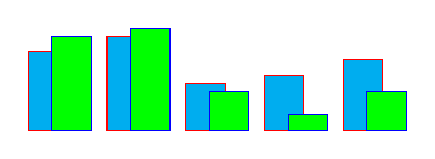
\begin{tikzpicture}[baseline=0pt]
\draw[red,fill=cyan,ybar,bar width=.5cm]plot coordinates{(0,1) (1,1.2) (2,.6) (3,.7) (4,.9)};
\draw[blue,fill=green,ybar,bar width=.5cm,bar shift=.3cm]plot coordinates{(0,1.2) (1,1.3) (2,.5) (3,.2) (4,.5)};
\end{tikzpicture}
&
\parbox[c]{10cm}{
\BS{begin}\AC{tikzpicture} \\
\BS{draw}[red,fill=cyan,ybar,bar width=.5cm] \\
\rule{1cm}{.0pt} plot coordinates \AC{(0,1) (1,1.2) (2,.6) (3,.7) (4,.9)}; \\
\BS{draw}[blue,fill=green,ybar,bar width=.5cm,\RDD{bar shift}=.3cm] \\
\rule{1cm}{.0pt} plot coordinates \AC{(0,1.2) (1,1.3) (2,.5) (3,.2) (4,.5)}; \\
\BS{end}\AC{tikzpicture} }
 \\  \hline 
 \end{tabular} 

\bigskip

\begin{tabular}{|c | c | c | c |c |} \hline
\multicolumn{4}{|c|}{ \BS{tikz} \BS{draw}  plot[xbar interval] file \AC{table.dat} ;   }\\ 
\hline
\tikz \draw[blue] plot[xbar] coordinates{(2,0) (3,1) (1,2) (2,3)};
&
\tikz \draw[blue] plot[xbar interval]  coordinates {(2,0) (3,1) (1,2) (2,3)};
&
\tikz \draw[blue] plot[xbar interval,x=.5cm]  coordinates {(2,0) (3,1) (1,2) (2,3)};
&
\tikz \draw[blue] plot[xbar interval,y=.5cm]  coordinates {(2,0) (3,1) (1,2) (2,3)};
%&
%\tikz \draw[blue!20] plot[xbar interval,x=.5cm,y=.5cm]  coordinates {(2,0) (3,1) (1,2) (2,3)};
\\ \hline
[\RDD{xbar}] & [\RDD{xbar interval}] & [xbar interval,\RDD{x}=.5cm] & [xbar interval,\RDD{y}=.5cm] 
\\ \hline
\end{tabular}

\newpage
%--------------------------------------------------------------
%\subsubsection{Graphe à partir d'une fonction}
\SbSbSSCT{Graphe à partir d'une fonction}{Graph of a function}


\begin{tabular}{|c | c | c | } \hline
\multicolumn{3}{|c|}{  \BS{draw}  [color=red] plot (\BS{x},\BS{x});   }\\ 
\hline
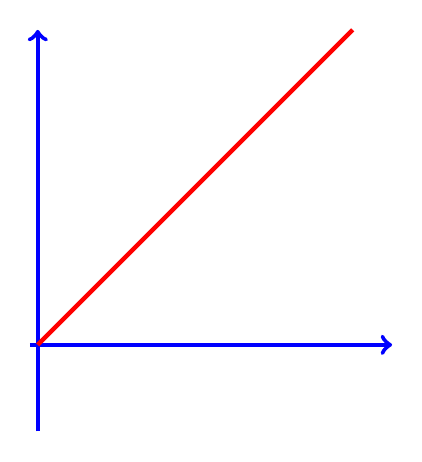
\begin{tikzpicture}[domain=0:4,ultra thick]
%\draw[very thin,color=gray] (-0.1,-1.1) grid (4.1,4.1);
\draw[->,blue,ultra thick] (-.1,0) -- (4.5,0);
\draw[->,blue,ultra thick] (0,-1.1) -- (0,04);
\draw[color=red] plot (\x,\x);
\end{tikzpicture} 
&
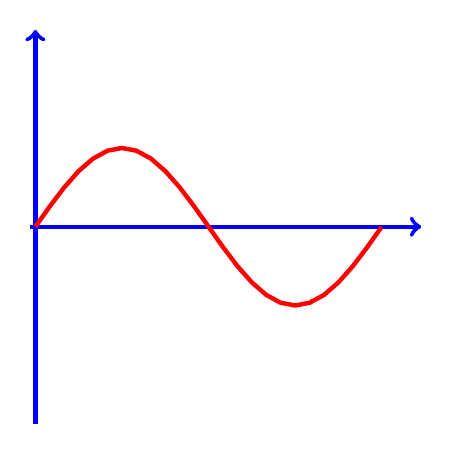
\begin{tikzpicture}[domain=0:6.28,ultra thick,x=0.7cm]
%\draw[very thin,color=gray] (-0.1,-2.1) grid (4.1,2.1);
\draw[->,blue,ultra thick] (-.1,0) -- (7,0);
\draw[->,blue,ultra thick] (0,-2.5) -- (0,2.5);
\draw[color=red] plot  (\x,{sin(\x r)});
\end{tikzpicture} 
&
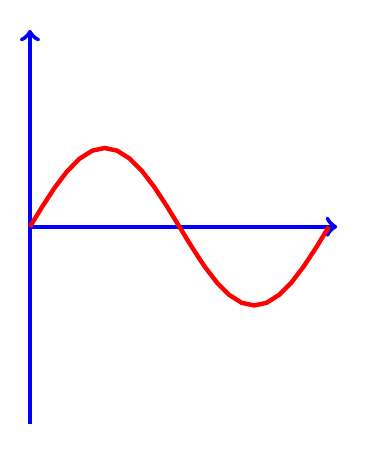
\begin{tikzpicture}[domain=0:360,x=0.3,ultra thick]
%\draw[very thin,color=gray] (-0.1,-2.1) grid (4.1,2.1);
\draw[->,blue,ultra thick] (-.1,0) -- (370,0);
\draw[->,blue,ultra thick] (0,-2.5) -- (0,2.5);
\draw[color=red] plot (\x,{sin(\x)});
\end{tikzpicture} 
\\ \hline
(\BS{x},\BS{x}) &  (\BS{x},\AC{sin(\BS{x} r)}) & (\BS{x},\AC{sin(\BS{x})}) \\
& x en radian & x en degré
\\ \hline
\end{tabular}

Options 

\begin{tabular}{|c | c |} \hline
\multicolumn{2}{|l|}{ \BS{draw}[color=red,dashed] plot(\BS{x},\AC{sin(\BS{x} r)});}  \\
\multicolumn{2}{|l|}{ \BS{draw}[color=blue,\RDD{samples}=5,mark=*,ultra thick] plot(\BS{x},\AC{sin(\BS{x} r)});} 
\\ \hline
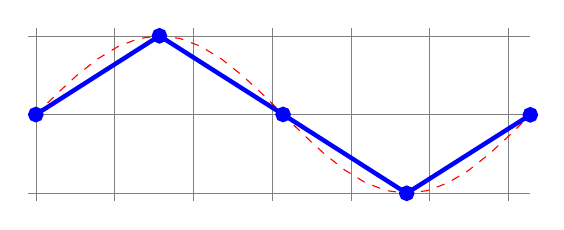
\begin{tikzpicture}[domain=0:6.28]
\draw[very thin,color=gray] (-0.1,-1.1) grid (6.28,1.1);
\draw[color=red,dashed] plot  (\x,{sin(\x r)});
\draw[color=blue,samples=5,mark=*,ultra thick] plot  (\x,{sin(\x r)});
\end{tikzpicture} 
&
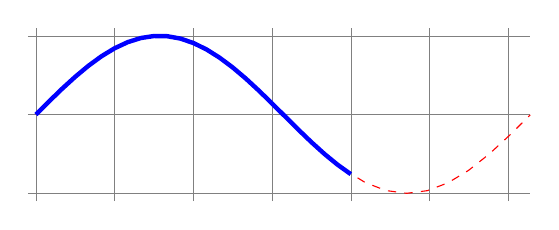
\begin{tikzpicture}
\draw[very thin,color=gray] (-0.1,-1.1) grid (6.28,1.1);
\draw[color=red,dashed,domain=0:6.28] plot  (\x,{sin(\x r)});
\draw[color=blue,domain=0:4,ultra thick] plot  (\x,{sin(\x r)});
\end{tikzpicture} 
  \\ \hline
[color=blue,\RDD{samples}=5,mark=*] & [color=blue,\RDD{domain}=0:4]
\\ \hline
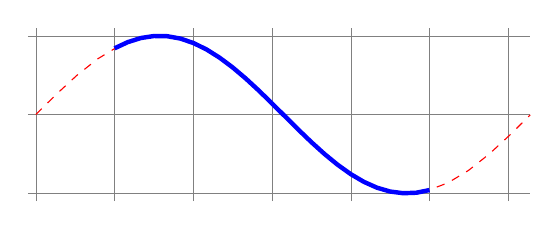
\begin{tikzpicture}
\draw[very thin,color=gray] (-0.1,-1.1) grid (6.28,1.1);
\draw[color=red,dashed,domain=0:6.28] plot  (\x,{sin(\x r)});
\draw[color=blue,domain=1:5,ultra thick] plot  (\x,{sin(\x r)});
\end{tikzpicture} 
&
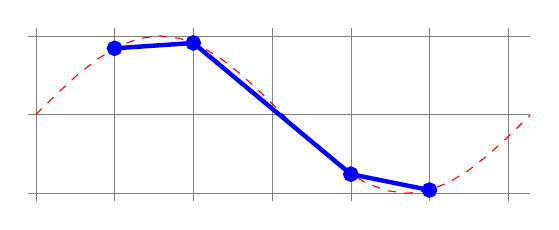
\begin{tikzpicture}[domain=0:6.28]
\draw[very thin,color=gray] (-0.1,-1.1) grid (6.28,1.1);
\draw[color=red,dashed] plot  (\x,{sin(\x r)});
\draw[color=blue,samples at={1,2,4,5},mark=*,ultra thick] plot  (\x,{sin(\x r)});
\end{tikzpicture} 
\\ \hline
[color=blue,\RDD{domain}=1:5] & [color=blue,\RDD{samples at}=\AC{1,2,4,5},mark=*]
\\ \hline
\end{tabular}


%-------------------------------------------------------------------------
%\subsubsection{Fonctions paramétriques}
\SbSbSSCT{Fonctions paramétriques}{Parametric function}


\begin{tabular}{|c | c |} \hline
\multicolumn{2}{|l|}{  \BS{draw}[domain=-3.141:3.141,smooth,variable=\BS{t}]plot (\AC{sin(\BS{t} r)},\AC{sin(2 *\BS{t} r)});} \\
\multicolumn{2}{|l|}{  \BS{draw}[domain=0:720,smooth,variable=\BS{t}]plot (\AC{sin(\BS{t})},\BS{t}/360,\AC{cos(\BS{t})});} 
\\ \hline

\tikz \draw[domain=-3.141:3.141,smooth,variable=\t,ultra thick]plot ({sin(\t r)},{sin(2*\t r)});
&
\tikz \draw[domain=0:720,smooth,variable=\t,ultra thick] plot ({sin(\t)},\t/360,{cos(\t)});
\\ \hline
(\AC{sin(\BS{t} r)},\AC{sin(2 *\BS{t} r)}) & (\AC{sin(\BS{t})},\BS{t}/360,\AC{cos(\BS{t})})
\\ \hline
\end{tabular} 
%\tikz \draw plot[mark=x,mark repeat=3,smooth] file {plots/pgfmanual-sine.table};
 

%\subsection{Marques}
\SbSSCT{Marques}{Marks}

%\subsubsection{Marques avec Tikz}
\SbSbSSCT{Marques avec TikZ}{Marks with TikZ}

\begin{tabular}{|c | c | c | c |} \hline
\tikz \draw plot[mark=+,mark size=5pt] coordinates {(0,0) (1,1) (2,0)};
&
\tikz \draw plot[mark=x,mark size=5pt] coordinates {(0,0) (1,1) (2,0) };
&
\tikz \draw plot[mark=*,mark size=5pt] coordinates {(0,0) (1,1) (2,0)};
&
\tikz \draw plot[mark=ball,mark size=5pt] coordinates {(0,0) (1,1) (2,0)};
\\ \hline
mark=+ & mark=x & mark=* & mark=ball
\\ \hline
\end{tabular}

\bigskip

\begin{tabular}{|c | c |} \hline
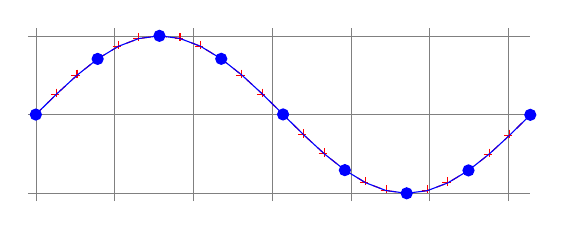
\begin{tikzpicture}[domain=0:6.28]
\draw[very thin,color=gray] (-0.1,-1.1) grid (6.28,1.1);
\draw[color=red,dashed,mark=+] plot  (\x,{sin(\x r)});
\draw[color=blue,mark repeat=3,mark=*] plot  (\x,{sin(\x r)});
\end{tikzpicture} 
&
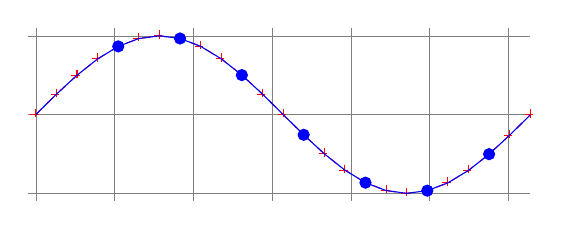
\begin{tikzpicture}[domain=0:6.28]
\draw[very thin,color=gray] (-0.1,-1.1) grid (6.28,1.1);
\draw[color=red,dashed,mark=+] plot  (\x,{sin(\x r)});
\draw[color=blue,mark repeat=3,mark phase=5,mark=*] plot  (\x,{sin(\x r)});
\end{tikzpicture} 
\\ \hline
[color=blue,\RDD{mark repeat}=3,mark=*] & [color=blue,mark repeat=3,\RDD{mark phase}=5,mark=*]
\\ \hline
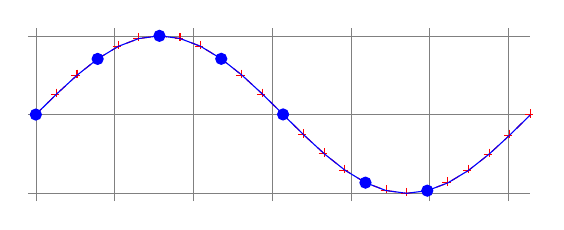
\begin{tikzpicture}[domain=0:6.28]
\draw[very thin,color=gray] (-0.1,-1.1) grid (6.28,1.1);
\draw[color=red,dashed,mark=+] plot  (\x,{sin(\x r)});
\draw[color=blue,mark indices={1,4,...,15,17,20},mark=*] plot  (\x,{sin(\x r)});
\end{tikzpicture} 
&
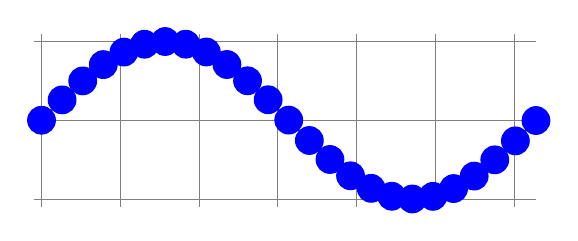
\begin{tikzpicture}[domain=0:6.28]
\draw[very thin,color=gray] (-0.1,-1.1) grid (6.28,1.1);
\draw[color=red,dashed,mark=+] plot  (\x,{sin(\x r)});
\draw[color=blue,mark size=5pt,mark=*] plot  (\x,{sin(\x r)});
\end{tikzpicture} 
\\ \hline
[color=blue,\RDD{mark indices}={1,4,...,15,17,20},mark=*] & [color=blue,\RDD{mark size}=5pt,mark=*]
\\ \hline
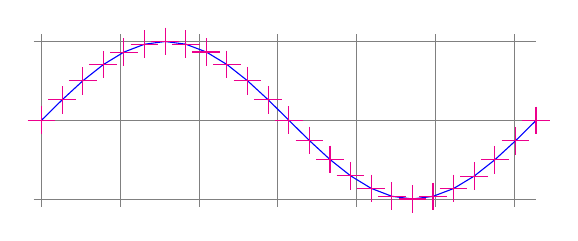
\begin{tikzpicture}[domain=0:6.28]
\draw[very thin,color=gray] (-0.1,-1.1) grid (6.28,1.1);
%\draw[color=red,dashed,mark=*] plot  (\x,{sin(\x r)});
\draw[color=blue,mark size=5pt,mark options={color=magenta},mark=+] plot  (\x,{sin(\x r)});
\end{tikzpicture}
&
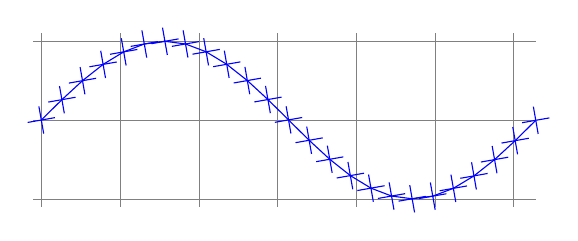
\begin{tikzpicture}[domain=0:6.28]
\draw[very thin,color=gray] (-0.1,-1.1) grid (6.28,1.1);
%\draw[color=red,dashed,mark=*] plot  (\x,{sin(\x r)});
\draw[color=blue,mark size=5pt,mark options={rotate=10},mark=+] plot  (\x,{sin(\x r)});
\end{tikzpicture}
\\ \hline
\RDD{mark options}=\AC{color=magenta},mark=+ & \RDD{mark options}=\AC{rotate=10},mark=+
\\ \hline
\end{tabular}
 

%\subsubsection{Marques personnalisées avec text mark}
\SbSbSSCT{Marques personnalisées avec text mark}{Marks with text mark}

\begin{tabular}{|c | c | c |} \hline
\multicolumn{3}{|l|}{ \BS{draw}[\RDD{mark=text},\RDD{text mark}=A,mark size=5pt] coordinates \AC{(0,0) (1,1) (2,0)};} 
\\ \hline
\tikz \draw plot[mark=text,text mark=A,mark size=5pt] coordinates {(0,0) (1,1) (2,0)};
&
\tikz \draw plot[mark=text,text mark=Texte,mark size=5pt] coordinates {(0,0) (1,1) (2,0)};
&
\begin{tikzpicture}
\draw[white]  (-1,0)-- (-1,1.5);
 \draw plot[mark=text,text mark=\DFR,mark size=5pt] coordinates {(0,0) (1,1) (2,0)};
\end{tikzpicture} 
\\ \hline
\RDD{text mark}=A &  \RDD{text mark}=Texte & \RDD{text mark}=\BS{DFR} \pageref{DFR} 
\\ \hline 
\multicolumn{3}{|c|}{ 
\begin{tikzpicture}
\draw[white]  (-1,0)-- (-1,1.5);
\draw plot[mark=text,text mark={\includegraphics[width=.5cm]{tiger}} ,mark size=5pt] coordinates {(0,0) (1,1) (2,0)};  
\end{tikzpicture} }
\\ \hline  
\multicolumn{3}{|c|}{ \RDD{text mark}=\AC{\BS{includegraphics}[width=.5cm]\AC{tiger}} }
\\ \hline   
\end{tabular}


\newpage
%\subsubsection{Marques avec l'extension plotmarks }
\SbSbSSCT{Marques avec l'extension plotmarks }{Marks with plotmarks library}

\label{plotmarks}

%Insérer dans le préambule :

 \maboite{\BS{usetikzlibrary}\AC{plotmarks}}
 
\begin{center}
\RRR{63}
\end{center}

\begin{tabular}{|c | c | c | c |} \hline
\tikz \draw plot[mark=-,mark size=5pt] coordinates {(0,0) (1,1) (2,0)};
& 
\tikz \draw plot[mark=|,mark size=5pt] coordinates {(0,0) (1,1) (2,0)};
 &
\tikz \draw plot[mark=o,mark size=5pt] coordinates {(0,0) (1,1) (2,0)};
 &
\tikz \draw plot[mark=asterisk,mark size=5pt] coordinates {(0,0) (1,1) (2,0)};
\\ \hline 
mark=- & mark=| & mark=o &mark=asterisk
\\ \hline
\tikz \draw plot[mark=star,mark size=5pt] coordinates {(0,0) (1,1) (2,0)};
&
\tikz \draw plot[mark=10-pointed star,mark size=5pt] coordinates {(0,0) (1,1) (2,0)};
&
\tikz \draw plot[mark=oplus,mark size=5pt] coordinates {(0,0) (1,1) (2,0)};
&
\tikz \draw plot[mark=oplus*,mark size=5pt] coordinates {(0,0) (1,1) (2,0)};
\\ \hline
mark=star & mark=10-pointed star & mark=oplus & mark=oplus*
\\ \hline
 
\tikz \draw plot[mark=otimes,mark size=5pt] coordinates {(0,0) (1,1) (2,0)};
&
\tikz \draw plot[mark=otimes*,mark size=5pt] coordinates {(0,0) (1,1) (2,0)};
&
\tikz \draw plot[mark=square,mark size=5pt] coordinates {(0,0) (1,1) (2,0)};
&
\tikz \draw plot[mark=square*,mark size=5pt] coordinates {(0,0) (1,1) (2,0)};
\\ \hline
 mark=otimes & mark=otimes* & mark=square & mark=square*
  \\ \hline
  
\tikz \draw plot[mark=triangle,mark size=5pt] coordinates {(0,0) (1,1) (2,0)};
& 
\tikz \draw plot[mark=triangle*,mark size=5pt] coordinates {(0,0) (1,1) (2,0)};
& 
\tikz \draw plot[mark=diamond,mark size=5pt]  coordinates {(0,0) (1,1) (2,0)};
 &
\tikz \draw plot[mark=diamond*,mark size=5pt] coordinates {(0,0) (1,1) (2,0)};
\\ \hline 
mark=triangle & mark=triangle* & mark=diamond & mark=diamond*
\\ \hline 

\tikz \draw plot[mark=halfdiamond*,mark size=5pt] coordinates {(0,0) (1,1) (2,0)};
 &
\tikz \draw plot[mark=halfsquare*,mark size=5pt] coordinates {(0,0) (1,1) (2,0)};
 &
\tikz \draw plot[mark=halfsquare right*,mark size=5pt] coordinates {(0,0) (1,1) (2,0)};
 &
\tikz \draw plot[mark=halfsquare left*,mark size=5pt] coordinates {(0,0) (1,1) (2,0)};
\\ \hline 
mark=halfdiamond* & mark=halfsquare* & mark=halfsquare right* & mark=halfsquare left*
\\ \hline 

\tikz \draw plot[mark=pentagon,mark size=5pt] coordinates {(0,0) (1,1) (2,0)};
 &
\tikz \draw plot[mark=pentagon*,mark size=5pt] coordinates {(0,0) (1,1) (2,0)};
 &
\tikz \draw plot[mark=Mercedes star,mark size=5pt] coordinates {(0,0) (1,1) (2,0)};
 &
\tikz \draw plot[mark=Mercedes star flipped,mark size=5pt] coordinates {(0,0) (1,1) (2,0)};
 \\ \hline
 mark=pentagon & mark=pentagon* & mark=Mercedes star & mark=Mercedes star flipped
 \\ \hline 
 
\tikz \draw plot[mark=halfcircle,mark size=5pt] coordinates {(0,0) (1,1) (2,0)};
 &
\tikz \draw plot[mark=halfcircle*,mark size=5pt] coordinates {(0,0) (1,1) (2,0)};
& 
\tikz \draw plot[mark=heart,mark size=5pt] coordinates {(0,0) (1,1) (2,0)};
 &
\tikz \draw plot[mark=text,mark size=5pt] coordinates {(0,0) (1,1) (2,0)};
 \\ \hline
 mark=halfcircle & mark=halfcircle* & mark=heart & mark=text
  \\ \hline
\end{tabular}

\bigskip

\begin{tabular}{|c | c | c | c |} \hline
\multicolumn{4}{|l|}{ \BS{draw}[mark=halfcircle,\RDD{mark color}=red,mark size=5pt] coordinates \AC{(0,0) (1,1) (2,0)};} 
\\ \hline
\tikz \draw plot[mark=halfcircle,mark color=red,mark size=5pt] coordinates {(0,0) (1,1) (2,0)};
&
\tikz \draw plot[mark=halfcircle*,mark color=red,mark size=5pt] coordinates {(0,0) (1,1) (2,0)};
&
\tikz \draw plot[mark=halfdiamond*,mark color=red,mark size=5pt] coordinates {(0,0) (1,1) (2,0)};
&
\tikz \draw plot[mark=halfsquare*,mark color=red,mark size=5pt] coordinates {(0,0) (1,1) (2,0)};
  \\ \hline
  mark=halfcircle & mark=halfcircle* & mark=halfdiamond* & mark=halfsquare*
   \\ \hline 
\end{tabular}



% \subsection{Graphes avec Gnuplot}
\SbSSCT{Graphes avec Gnuplot}{Graph with Gnuplot}
 
 \begin{tabular}{|l| } \hline
%\begin{tikzpicture}[domain=0:6.28]
%%\draw[very thin,color=gray] (-0.1,-1.1) grid (7.1,1.1);
%%\draw[->,ultra thick,blue] (-0.2,0) -- (7,0) node[right] {$x$};
%%\draw[->,ultra thick,blue] (0,-1.2) -- (0,1.2) node[above] {$f(x)$};
%%\draw[color=red] plot[id=x] function{x} node[right] {$f(x) =x$};
%\draw[color=red] plot[id=sin] function{sin(x)} ;
%%\draw[color=orange] plot[id=exp] function{0.05*exp(x)} node[right] {$f(x) = \frac{1}{20} \mathrm e^x$};
%\end{tikzpicture}
\BS{draw}[color=red] plot[\RDD{id}=sin] function\AC{sin(x)} ;
   \\ \hline
\\
==> plot[id=sin] \TFRGB{crée le fichier}{create the file} \og sin.gnuplot \fg \\
==>  \TFRGB{Ouvrir le fichier}{Open the file} \og sin.gnuplot \fg \TFRGB{avec le programme gnuplot pour créer le fichier}{with the program gnuplot : creation of the file }   \og sin.table \fg\\
==> \TFRGB{Utiliser le fichier de données} {Use the datafile }
 \og sin.table  \fg   \\ \hline 
\end{tabular}